\documentclass{ximera}

\input{../../../preamble.tex}


\definecolor{fvdnavy}{HTML}{071D43}
\definecolor{fvdcyan}{HTML}{20BFC6}
\definecolor{fvdcyanlight}{HTML}{EFFCFB}
\definecolor{fvdmagenta}{HTML}{F10D69}
\definecolor{fvdmagentalight}{HTML}{FFF1F7}
\definecolor{fvdtext}{HTML}{163044}





%=================================================
% Pedagogische omgevingen
% PDF: tcolorbox
% HTML: learning-box
%=================================================

\newenvironment{voorkennis}
{%
    \ifdefined\HCode
        \HCode{%
<section class="learning-box learning-box--prior">
<div class="learning-box__header">
<span class="learning-box__icon" aria-hidden="true"></span>
<span class="learning-box__title">Voorkennis</span>
</div>
<div class="learning-box__content">
        }%
        \begin{itemize}
    \else
       \begin{tcolorbox}[
    enhanced,
    breakable,
    colback=fvdcyanlight,
    colframe=fvdcyan,
    coltext=fvdtext,
    boxrule=0.5pt,
    leftrule=4pt,
    arc=4mm,
    outer arc=4mm,
    left=7mm,
    right=6mm,
    top=5mm,
    bottom=5mm,
    before skip=6mm,
    after skip=6mm,
    title=Voorkennis,
    coltitle=fvdcyan,
    fonttitle=\bfseries\Large,
    attach title to upper={\par\smallskip},
    boxed title style={
        empty,
        left=0mm,
        right=0mm,
        top=0mm,
        bottom=0mm
    },
    overlay={
        \draw[
            fvdcyan,
            line width=0.5pt
        ]
        ([xshift=42mm,yshift=-13mm]frame.north west)
        --
        ([xshift=-7mm,yshift=-13mm]frame.north east);
    }
]
        \begin{itemize}
    \fi
}
{%
    \end{itemize}
    \ifdefined\HCode
        \HCode{%
</div>
</section>
        }%
    \else
        \end{tcolorbox}
    \fi
}


\newenvironment{leerdoelen}
{%
    \ifdefined\HCode
        \HCode{%
<section class="learning-box learning-box--goals">
<div class="learning-box__header">
<span class="learning-box__icon" aria-hidden="true"></span>
<span class="learning-box__title">Leerdoelen</span>
</div>
<div class="learning-box__content">
        }%
        \begin{itemize}
    \else
\begin{tcolorbox}[
    enhanced,
    breakable,
    colback=fvdmagentalight,
    colframe=fvdmagenta,
    coltext=fvdtext,
    boxrule=0.5pt,
    leftrule=4pt,
    arc=4mm,
    outer arc=4mm,
    left=7mm,
    right=6mm,
    top=5mm,
    bottom=5mm,
    before skip=6mm,
    after skip=6mm,
    title=Leerdoelen,
    coltitle=fvdmagenta,
    fonttitle=\bfseries\Large,
    attach title to upper={\par\smallskip},
    boxed title style={
        empty,
        left=0mm,
        right=0mm,
        top=0mm,
        bottom=0mm
    },
    overlay={
        \draw[
            fvdmagenta,
            line width=0.5pt
        ]
        ([xshift=42mm,yshift=-13mm]frame.north west)
        --
        ([xshift=-7mm,yshift=-13mm]frame.north east);
    }
]
        \begin{itemize}
    \fi
}
{%
    \end{itemize}
    \ifdefined\HCode
        \HCode{%
</div>
</section>
        }%
    \else
        \end{tcolorbox}
    \fi
}


\addPrintStyle{../../..}

\title{Oefeningen — Van relatie naar functie}
\author{Ingmar Herreman}

\begin{document}

% FVD_CHAPTER_DATA_START
% Automatisch gegenereerd uit index.tex.
% Niet handmatig aanpassen.
\fvdchapterdata{4}{Van relatie naar functie}{1}
% FVD_CHAPTER_DATA_END









\maketitle

\FVDbeginExercises

% ============================================================
% BASIS
% ============================================================



\begin{oefening}[Afhankelijk of onafhankelijk?]{\oefB\ESS}

Bepaal telkens een zinvolle onafhankelijke en afhankelijke grootheid.
Motiveer kort.

\begin{question}
De inhoud van een cilindervormig vat wordt onderzocht voor verschillende
vulhoogten.

\begin{oplossing}
Een natuurlijke keuze is:
\[
\text{onafhankelijk: vulhoogte }h,
\qquad
\text{afhankelijk: volume }V.
\]
Bij een gegeven vulhoogte ligt het volume vast.
\end{oplossing}
\end{question}

\begin{question}
Een temperatuursensor registreert iedere seconde de temperatuur van een proefmonster.

\begin{oplossing}
\[
\text{onafhankelijk: tijd }t,
\qquad
\text{afhankelijk: temperatuur }T.
\]
\end{oplossing}
\end{question}

\begin{question}
Voor cirkels wordt de oppervlakte onderzocht in functie van de straal.

\begin{oplossing}
\[
\text{onafhankelijk: straal }r,
\qquad
\text{afhankelijk: oppervlakte }A.
\]
\end{oplossing}
\end{question}

\end{oefening}

% ------------------------------------------------------------

\begin{oefening}[Functie of geen functie? — pijldiagrammen]{\oefB\ESS}

Onderzoek elk diagram. Is de relatie een functie van de linker naar de rechter
verzameling? Motiveer vanuit de definitie.

\begin{question}

\begin{center}
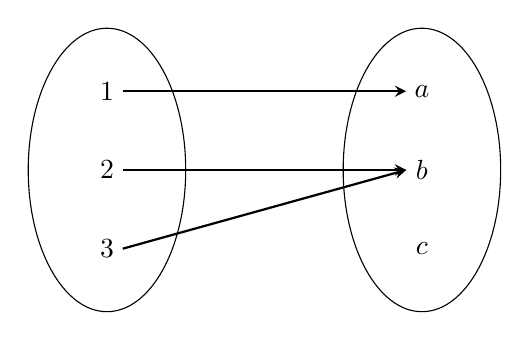
\begin{tikzpicture}[>=stealth]
\draw (-2,0) ellipse (1 and 1.8);
\draw (2,0) ellipse (1 and 1.8);
\node at (-2,1) {$1$};
\node at (-2,0) {$2$};
\node at (-2,-1) {$3$};
\node at (2,1) {$a$};
\node at (2,0) {$b$};
\node at (2,-1) {$c$};
\draw[->,thick] (-1.8,1)--(1.8,1);
\draw[->,thick] (-1.8,0)--(1.8,0);
\draw[->,thick] (-1.8,-1)--(1.8,0);
\end{tikzpicture}
\end{center}

\begin{oplossing}
Ja. Iedere invoerwaarde \(1,2,3\) heeft precies één uitvoerwaarde.
Dat \(2\) en \(3\) eventueel dezelfde uitvoer zouden hebben, vormt geen probleem.
\end{oplossing}
\end{question}

\begin{question}

\begin{center}
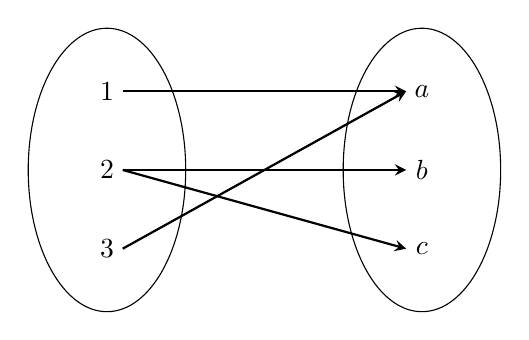
\begin{tikzpicture}[>=stealth]
\draw (-2,0) ellipse (1 and 1.8);
\draw (2,0) ellipse (1 and 1.8);
\node at (-2,1) {$1$};
\node at (-2,0) {$2$};
\node at (-2,-1) {$3$};
\node at (2,1) {$a$};
\node at (2,0) {$b$};
\node at (2,-1) {$c$};
\draw[->,thick] (-1.8,1)--(1.8,1);
\draw[->,thick] (-1.8,0)--(1.8,0);
\draw[->,thick] (-1.8,0)--(1.8,-1);
\draw[->,thick] (-1.8,-1)--(1.8,1);
\end{tikzpicture}
\end{center}

\begin{oplossing}
Nee. Bij invoer \(2\) horen twee verschillende uitvoerwaarden, namelijk \(b\) en \(c\).
\end{oplossing}
\end{question}

\end{oefening}

% ------------------------------------------------------------

\begin{oefening}[Functie of geen functie? — tabellen en koppels]{\oefB\ESS}

\begin{question}
Onderzoek de tabel.

\[
\begin{array}{c|ccccc}
x&-2&-1&0&1&2\\
\hline
y&4&1&0&1&4
\end{array}
\]

\begin{oplossing}
Dit is een functie: bij iedere gegeven \(x\)-waarde hoort precies één \(y\)-waarde.
Dat verschillende \(x\)-waarden dezelfde \(y\)-waarde hebben, is toegestaan.
\end{oplossing}
\end{question}

\begin{question}
Onderzoek de relatie
\[
R=\{(-2,4),(-1,1),(0,0),(1,1),(1,3)\}.
\]

\begin{oplossing}
Geen functie van \(x\) naar \(y\), want bij \(x=1\) horen twee verschillende
uitvoerwaarden: \(1\) en \(3\).
\end{oplossing}
\end{question}

\begin{question}
Onderzoek de relatie
\[
R=\{(1,5),(2,5),(3,5),(4,5)\}.
\]

\begin{oplossing}
Dit is wel een functie. Iedere invoer heeft precies één uitvoer.
Alle invoerwaarden mogen dezelfde uitvoerwaarde \(5\) hebben.
\end{oplossing}
\end{question}

\end{oefening}

% ------------------------------------------------------------

\begin{oefening}[De verticale-lijntest]{\oefB\ESS}

Bepaal voor elke grafiek of \(y\) een functie van \(x\) is.
Verantwoord met de verticale-lijntest.

\begin{question}

\begin{center}
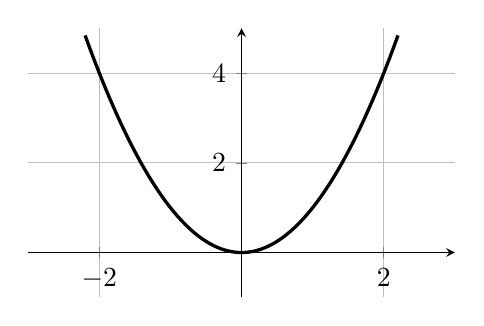
\begin{tikzpicture}
\begin{axis}[
width=7cm,height=5cm,
xmin=-3,xmax=3,ymin=-1,ymax=5,
axis lines=middle,grid=both,samples=120]
\addplot[very thick,domain=-2.2:2.2] {x^2};
\end{axis}
\end{tikzpicture}
\end{center}

\begin{oplossing}
Ja. Iedere verticale lijn snijdt de grafiek hoogstens eenmaal.
\end{oplossing}
\end{question}

\begin{question}

\begin{center}
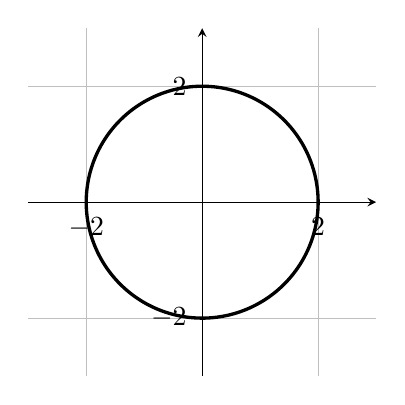
\begin{tikzpicture}
\begin{axis}[
width=7cm,height=6cm,
xmin=-3,xmax=3,ymin=-3,ymax=3,
axis lines=middle,grid=both,axis equal image]
\addplot[very thick,domain=0:360,samples=180] ({2*cos(x)},{2*sin(x)});
\end{axis}
\end{tikzpicture}
\end{center}

\begin{oplossing}
Nee. Voor veel \(x\)-waarden snijdt een verticale lijn de cirkel tweemaal.
\end{oplossing}
\end{question}

\begin{question}

\begin{center}
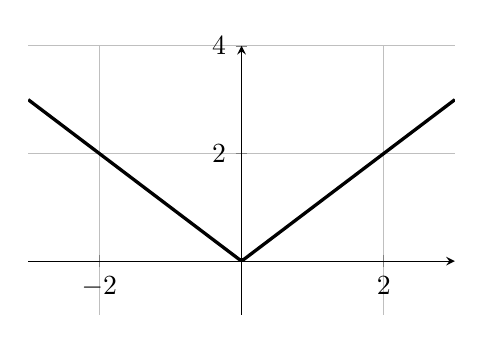
\begin{tikzpicture}
\begin{axis}[
width=7cm,height=5cm,
xmin=-3,xmax=3,ymin=-1,ymax=4,
axis lines=middle,grid=both,samples=120]
\addplot[very thick,domain=-3:3] {abs(x)};
\end{axis}
\end{tikzpicture}
\end{center}

\begin{oplossing}
Ja. Iedere verticale lijn snijdt de grafiek hoogstens eenmaal.
\end{oplossing}
\end{question}

\end{oefening}

% ------------------------------------------------------------

\begin{oefening}[Functienotatie]{\oefB\ESS}

Gegeven is
\[
f(x)=2x^2-3x-1.
\]

\begin{question}
Bereken \(f(0)\), \(f(2)\) en \(f(-1)\).

\begin{oplossing}
\[
f(0)=-1,
\]
\[
f(2)=2\cdot4-6-1=1,
\]
\[
f(-1)=2\cdot1+3-1=4.
\]
\end{oplossing}
\end{question}

\begin{question}
Geef drie punten die zeker op de grafiek van \(f\) liggen.

\begin{oplossing}
Bijvoorbeeld
\[
(0,-1),\qquad (2,1),\qquad (-1,4).
\]
\end{oplossing}
\end{question}

\begin{question}
Leg in één zin uit wat het verschil is tussen \(f\) en \(f(2)\).

\begin{oplossing}
\(f\) is de functie zelf, terwijl \(f(2)\) de functiewaarde is die hoort bij invoer \(2\).
\end{oplossing}
\end{question}

\end{oefening}

% ------------------------------------------------------------

\begin{oefening}[Van voorschrift naar tabel en grafiek]{\oefB\ESS}

Een tank bevat aanvankelijk \(10\) liter water en wordt gevuld met
\(2\) liter per minuut. Het model is

\[
V(t)=10+2t.
\]

\begin{question}
Vul de tabel aan.

\[
\begin{array}{c|ccccc}
t\;(\mathrm{min})&0&2&5&8&12\\
\hline
V\;(\mathrm{L})&&&&&
\end{array}
\]

\begin{oplossing}
\[
\begin{array}{c|ccccc}
t\;(\mathrm{min})&0&2&5&8&12\\
\hline
V\;(\mathrm{L})&10&14&20&26&34
\end{array}
\]
\end{oplossing}
\end{question}

\begin{question}
Teken de grafiek voor \(0\leq t\leq 12\).

\begin{oplossing}
De grafiek is het relevante lijnstuk van de rechte \(V=10+2t\), beginnend
in \((0,10)\) en eindigend in \((12,34)\).
\end{oplossing}
\end{question}

\begin{question}
Wat betekent \(V(12)=34\) in de context?

\begin{oplossing}
Na \(12\) minuten bevat de tank volgens het model \(34\) liter water.
\end{oplossing}
\end{question}

\end{oefening}

% ============================================================
% VERDIEPING
% ============================================================



\begin{oefening}[Een cirkel: relatie maar geen functie]{\oefU\ESS}

Beschouw
\[
x^2+y^2=25.
\]

\begin{question}
Leg zonder grafiek uit waarom \(y\) geen functie van \(x\) is op de volledige cirkel.

\begin{oplossing}
Uit
\[
x^2+y^2=25
\]
volgt
\[
y=\pm\sqrt{25-x^2}.
\]
Voor bijvoorbeeld \(x=0\) zijn er twee mogelijke waarden:
\[
y=5\quad\text{en}\quad y=-5.
\]
Dus één invoer kan twee uitvoerwaarden hebben.
\end{oplossing}
\end{question}

\begin{question}
Teken de cirkel in GeoGebra en controleer je redenering met een beweegbare verticale lijn.

\begin{oplossing}
Voor alle \(x\)-waarden strikt tussen \(-5\) en \(5\) snijdt de verticale lijn
de cirkel doorgaans in twee punten.
\end{oplossing}
\end{question}

\end{oefening}

% ------------------------------------------------------------

\begin{oefening}[GeoGebra-onderzoek: functie of niet?]{\oefU\ESS}

Gebruik GeoGebra. Onderzoek de volgende relaties:

\[
y=x^3-x,\qquad
y^2=x+2,\qquad
x^2+y^2=9,\qquad
y=|x-1|.
\]

Maak een schuifknop \(a\) en teken \(x=a\).

\begin{question}
Classificeer elke relatie als ``functie van \(x\)'' of ``geen functie van \(x\)''.

\begin{oplossing}
\[
y=x^3-x:\ \text{functie},
\]
\[
y^2=x+2:\ \text{geen functie},
\]
\[
x^2+y^2=9:\ \text{geen functie},
\]
\[
y=|x-1|:\ \text{functie}.
\]
\end{oplossing}
\end{question}

\begin{question}
Geef voor elke relatie die geen functie is één concrete \(x\)-waarde
waarvoor je twee verschillende \(y\)-waarden vindt.

\begin{oplossing}
Voor \(y^2=x+2\) kan bijvoorbeeld \(x=2\):
\[
y^2=4\Rightarrow y=\pm2.
\]

Voor de cirkel kan bijvoorbeeld \(x=0\):
\[
y^2=9\Rightarrow y=\pm3.
\]
\end{oplossing}
\end{question}

\begin{question}
Leg uit waarom de GeoGebra-constructie met \(x=a\) precies de definitie
van een functie test.

\begin{oplossing}
De lijn \(x=a\) fixeert één invoerwaarde. Twee snijpunten met verschillende
hoogten betekenen dat dezelfde invoer \(a\) twee verschillende uitvoerwaarden krijgt.
Dat is in strijd met de definitie van een functie.
\end{oplossing}
\end{question}

\end{oefening}

% ------------------------------------------------------------

\begin{oefening}[Van context naar model en terug]{\oefU\ESS}

Een robot rijdt met constante snelheid langs een rechte baan.
Op \(t=0\) bevindt hij zich \(1{,}5\) meter rechts van een referentiepunt.
Hij rijdt verder naar rechts met \(0{,}60\ \mathrm{m/s}\).

\begin{question}
Stel een functievoorschrift \(x(t)\) op.

\begin{oplossing}
\[
x(t)=1{,}5+0{,}60t.
\]
\end{oplossing}
\end{question}

\begin{question}
Bereken \(x(4)\) en interpreteer het resultaat volledig.

\begin{oplossing}
\[
x(4)=1{,}5+0{,}60\cdot4=3{,}9.
\]
Na \(4\) seconden bevindt de robot zich volgens het model
\(3{,}9\) meter rechts van het referentiepunt.
\end{oplossing}
\end{question}

\begin{question}
Maak een tabel voor \(t=0,1,2,3,4\) en teken de grafiek.

\begin{oplossing}
\[
\begin{array}{c|ccccc}
t&0&1&2&3&4\\
\hline
x(t)&1{,}5&2{,}1&2{,}7&3{,}3&3{,}9
\end{array}
\]
De grafiek is een stijgend lijnstuk of een deel van de rechte
\(x=1{,}5+0{,}60t\), afhankelijk van het onderzochte tijdsinterval.
\end{oplossing}
\end{question}

\end{oefening}

% ------------------------------------------------------------

\begin{oefening}[Een bal in de lucht]{\oefU\ESS}

De hoogte van een bal wordt tijdens een worp gemodelleerd door

\[
h(t)=1{,}5+8t-4{,}905t^2,
\]

met \(h\) in meter en \(t\) in seconde.

\begin{question}
Bereken \(h(0)\), \(h(0{,}5)\) en \(h(1)\).

\begin{oplossing}
\[
h(0)=1{,}5,
\]
\[
h(0{,}5)=1{,}5+4-4{,}905\cdot0{,}25
=4{,}27375,
\]
\[
h(1)=1{,}5+8-4{,}905=4{,}595.
\]
\end{oplossing}
\end{question}

\begin{question}
Teken de grafiek met GeoGebra.

\begin{oplossing}
De grafiek is een neerwaarts gerichte parabool. In de fysische context
gebruiken we alleen het tijdsinterval waarin de beweging wordt beschreven.
\end{oplossing}
\end{question}

\begin{question}
Leg uit waarom negatieve waarden van \(t\) wiskundig in het voorschrift
kunnen worden ingevuld, maar in dit model niet noodzakelijk zinvol zijn.

\begin{oplossing}
Het algebraïsche voorschrift kan voor negatieve \(t\) worden berekend,
maar \(t\) stelt de verstreken tijd sinds het begin van de meting voor.
Negatieve verstreken tijd hoort niet bij de beschreven situatie.
\end{oplossing}
\end{question}

\end{oefening}

% ------------------------------------------------------------

\begin{oefening}[Foutenanalyse]{\oefU\ESS}

Een leerling zegt:

\begin{center}
``Als twee verschillende \(x\)-waarden dezelfde \(y\)-waarde hebben,
dan is de relatie geen functie.''
\end{center}

\begin{question}
Is de uitspraak juist? Motiveer.

\begin{oplossing}
Nee. Een functie vereist dat iedere invoer precies één uitvoer heeft.
Verschillende invoerwaarden mogen dezelfde uitvoer hebben.
Bijvoorbeeld \(f(x)=x^2\) heeft \(f(-2)=f(2)=4\) en is toch een functie.
\end{oplossing}
\end{question}

\begin{question}
Teken een grafiek die duidelijk laat zien waarom de uitspraak fout is.

\begin{oplossing}
Bijvoorbeeld de parabool \(y=x^2\).
De horizontale lijn \(y=4\) snijdt de grafiek tweemaal, maar iedere verticale
lijn snijdt de grafiek hoogstens eenmaal.
\end{oplossing}
\end{question}

\end{oefening}

% ============================================================
% GEVORDERD
% ============================================================



\begin{oefening}[Welke grootheid kies je als invoer?]{\oefG}

Een fietser rijdt een heuvelachtig parcours. Tijdens de rit passeert hij
dezelfde hoogte boven zeeniveau meerdere keren.

\begin{question}
Is de hoogte \(h\) een functie van de tijd \(t\)? Licht toe.

\begin{oplossing}
Ja, op ieder tijdstip bevindt de fietser zich op precies één hoogte.
Dus \(t\mapsto h(t)\) is een functie.
\end{oplossing}
\end{question}

\begin{question}
Is de tijd \(t\) noodzakelijk een functie van de hoogte \(h\)?
Licht toe.

\begin{oplossing}
Nee. De fietser kan dezelfde hoogte op verschillende tijdstippen passeren.
Eén hoogtewaarde kan dus met meerdere tijdstippen overeenkomen.
\end{oplossing}
\end{question}

\begin{question}
Wat leert dit voorbeeld over de richting waarin we een relatie bekijken?

\begin{oplossing}
Of een relatie een functie is, hangt af van welke grootheid als invoer
en welke als uitvoer wordt gekozen. Een verband kan in de ene richting
een functie zijn en in de omgekeerde richting niet.
\end{oplossing}
\end{question}

\end{oefening}

% ------------------------------------------------------------

\begin{oefening}[Ontwerp zelf een tegenvoorbeeld]{\oefG}

Construeer zelf:

\begin{enumerate}
    \item een relatie met vier invoerwaarden die een functie is,
          maar waarbij minstens twee invoerwaarden dezelfde uitvoer hebben;
    \item een relatie met vier invoerwaarden die geen functie is omdat één invoer
          twee verschillende uitvoerwaarden heeft;
    \item een grafiek die geen functie van \(x\) is, maar waarvan een deel wél
          een functie van \(x\) vormt.
\end{enumerate}

Geef telkens een korte verantwoording vanuit de definitie.

\begin{oplossing}
Er zijn veel mogelijke antwoorden.

Voorbeelden:

\[
\{(1,a),(2,a),(3,b),(4,c)\}
\]
is een functie.

\[
\{(1,a),(2,a),(2,b),(3,c),(4,c)\}
\]
is geen functie omdat invoer \(2\) twee uitvoerwaarden heeft.

Een volledige cirkel is geen functie van \(x\), maar de bovenste halve cirkel
\[
y=\sqrt{r^2-x^2}
\]
is wel een functie op het passende interval.
\end{oplossing}

\end{oefening}

% ------------------------------------------------------------

\begin{oefening}[Sensorgegevens onderzoeken]{\oefG}

Een sensor levert tijdens een proef de volgende meetgegevens:

\[
\begin{array}{c|cccccc}
t\;(\mathrm{s})&0&1&2&3&4&5\\
\hline
U\;(\mathrm{V})&0{,}42&0{,}56&0{,}71&0{,}85&1{,}01&1{,}14
\end{array}
\]

\begin{question}
Waarom kunnen deze gegevens worden opgevat als een functie \(U(t)\)?

\begin{oplossing}
Aan elk geregistreerd tijdstip in de tabel is precies één gemeten
spanningswaarde gekoppeld.
\end{oplossing}
\end{question}

\begin{question}
Voer de gegevens in GeoGebra in en maak een puntenwolk.
Beschrijf wat je ziet zonder meteen een exact voorschrift te veronderstellen.

\begin{oplossing}
De spanning neemt toe wanneer de tijd toeneemt. De punten lijken ongeveer
langs een stijgende rechte te liggen, maar op basis van meetgegevens alleen
hoeft het verband niet exact lineair te zijn.
\end{oplossing}
\end{question}

\begin{question}
Leg uit waarom ``de punten lijken op een rechte te liggen'' niet hetzelfde is
als ``de werkelijkheid is exact lineair''.

\begin{oplossing}
Een wiskundig model is een vereenvoudigde beschrijving van meetgegevens.
Meetfouten, beperkte meetnauwkeurigheid en een mogelijk niet-lineair fysisch
proces kunnen ervoor zorgen dat een rechte slechts een benadering is.
\end{oplossing}
\end{question}

\end{oefening}



\end{document}
